\chapter{Sviluppo di sistemi interattivi}
Nel mondo del design di sistemi interattivi, la metodologia utilizzata per gestire il progetto è cruciale per determinare il successo del prodotto finale. Esistono vari modelli di gestione dei progetti, ma due delle metodologie più ampiamente utilizzate sono il modello Waterfall e il metodo Agile. Ciascuno di questi approcci ha caratteristiche uniche, vantaggi e svantaggi, e viene scelto in base alla natura del progetto e alle esigenze del team.

\section{Modello waterfall}
Il modello Waterfall (a cascata) è uno dei modelli più tradizionali e segue una sequenza lineare e ben definita. Ogni fase deve essere completata prima che la successiva possa iniziare, creando una struttura rigida e chiara per lo sviluppo del progetto. 

\begin{figure}[ht]
    \centering
    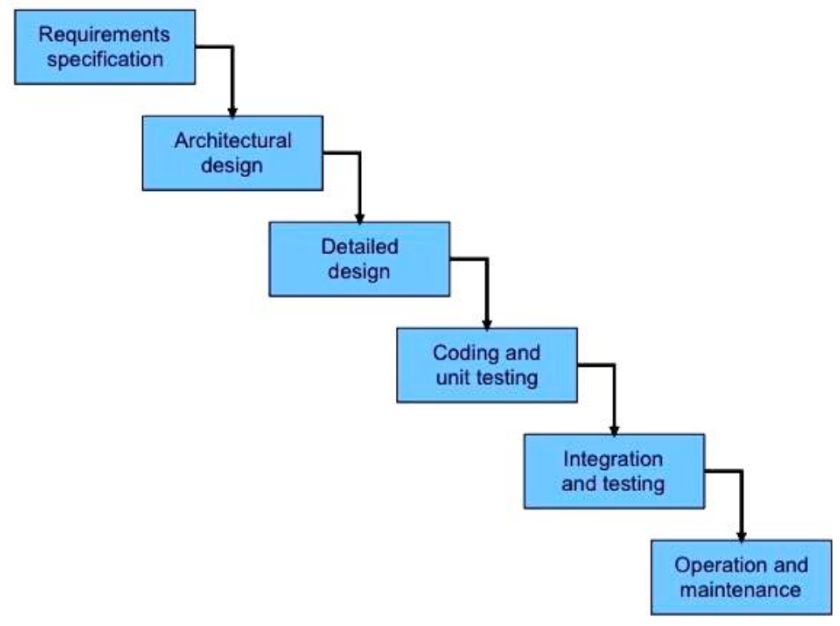
\includegraphics[width=0.6\linewidth]{images/waterfall-model.PNG}
    \caption{Modelo waterfall}
    \label{fig:waterfall-model}
\end{figure}

Le fasi principali del modello Waterfall includono:
\begin{enumerate}
    \item \textit{Analisi dei requisiti:} in questa fase vengono raccolti i requisiti dettagliati del sistema, definendo cosa deve fare il sistema e quali sono le aspettative degli utenti.
    \item \textit{Progettazione:} una volta definiti i requisiti, si passa alla progettazione del sistema, dove viene creato un modello dettagliato che includa aspetti come l'architettura del sistema e il design dell'interfaccia utente.
    \item \textit{Implementazione:} il sistema viene costruito seguendo il progetto definito, con gli sviluppatori che traducono il design in codice.
    \item \textit{Testing:} una volta completato lo sviluppo, il sistema viene testato per verificare che funzioni correttamente e soddisfi i requisiti stabiliti.
    \item \textit{Manutenzione:} dopo il rilascio, il sistema entra in fase di manutenzione, in cui vengono apportati miglioramenti e corretti eventuali bug.
\end{enumerate}
Un vantaggio del modello Waterfall è la sua struttura chiara: le fasi sequenziali e ben definite lo rendono ideale per progetti in cui i requisiti sono stabili e non prevedono cambiamenti significativi durante lo sviluppo. Tuttavia, la rigidità del Waterfall può essere uno svantaggio in contesti in cui è richiesta flessibilità, poiché ogni modifica nei requisiti implica la ripetizione di diverse fasi.

\begin{figure}[ht]
    \centering
    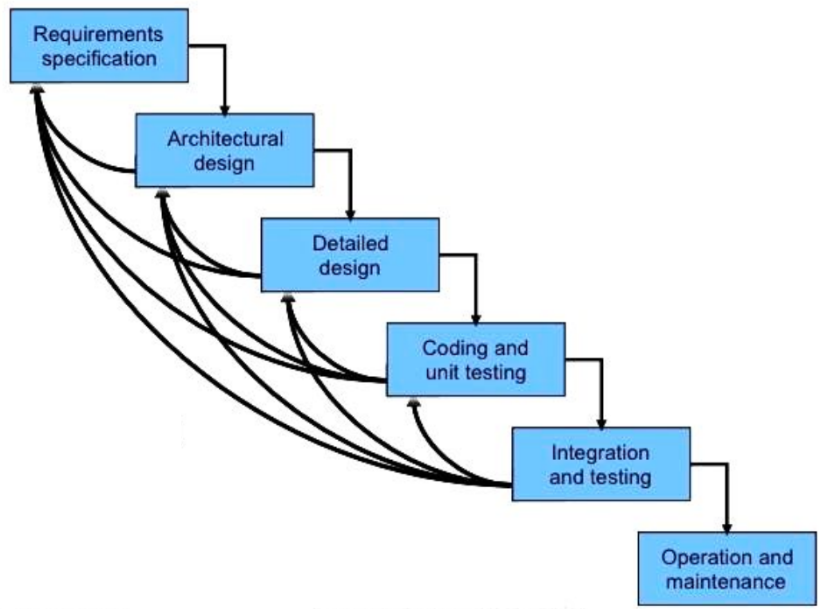
\includegraphics[width=0.6\linewidth]{images/life-cycle.PNG}
    \caption{Ciclo di vita per sistemi interattivi}
    \label{fig:life-cycle}
\end{figure}

\section{Metodo agile}
Il metodo Agile è stato introdotto per rispondere alla necessità di maggiore flessibilità nel processo di sviluppo. A differenza del modello Waterfall, Agile suddivide il progetto in cicli iterativi e incrementali chiamati sprint. Ogni sprint rappresenta una breve fase di sviluppo in cui vengono progettate, sviluppate e testate funzionalità specifiche. Alla fine di ogni sprint, il team verifica i progressi fatti, raccoglie feedback e adatta il progetto alle esigenze emergenti.

Le caratteristiche principali del metodo Agile includono:
\begin{itemize}
    \item \textit{Iterazione continua:} ogni ciclo fornisce un prodotto funzionante con nuove funzionalità o miglioramenti.
    \item \textit{Collaborazione costante con gli utenti:} il feedback viene raccolto alla fine di ogni sprint, consentendo aggiustamenti immediati.
    \item \textit{Flessibilità e adattabilità:} i team possono rispondere rapidamente ai cambiamenti nei requisiti e agli input degli stakeholder.
\end{itemize}
Agile si basa su quattro principi fondamentali:
\begin{enumerate}
    \item Focus sugli individui e le interazioni piuttosto che sui processi e strumenti.
    \item Software funzionante più che documentazione dettagliata.
    \item Collaborazione con il cliente più che negoziazione del contratto.
    \item Risposta al cambiamento più che seguire un piano fisso.
\end{enumerate}
Questi principi mettono l’accento sull’adattabilità e sulla capacità di rispondere rapidamente a nuove esigenze, rendendo Agile ideale per progetti complessi e dinamici in cui le specifiche possono cambiare nel tempo.

\subsection{Agile UDC}
La progettazione di sistemi interattivi richiede oggi un approccio che coniughi il metodo Agile con i principi del User-Centered Design (UCD). Mentre Agile offre flessibilità e iterazione continua, UCD assicura che il design sia incentrato sui bisogni degli utenti. Questo connubio tra Agile e UCD permette di creare sistemi che rispondano ai requisiti in modo dinamico, mantenendo sempre al centro l'esperienza utente.

Integrare Agile e UCD significa bilanciare l’attenzione sull’utente finale con la necessità di flessibilità del progetto. In un contesto Agile UCD, i team lavorano su brevi sprint che includono non solo fasi di sviluppo ma anche test e valutazioni con gli utenti. In ogni ciclo, si creano prototipi e versioni preliminari del sistema, che vengono testate dagli utenti e modificate secondo il feedback raccolto. Questo approccio riduce i rischi di progettazione, permettendo correzioni frequenti e incrementali basate su dati reali.

La combinazione di Agile e UCD richiede strumenti e processi che facilitino la collaborazione tra sviluppatori, designer e utenti. Ad esempio, per mantenere l’attenzione sull’utente, si utilizzano frequentemente storyboards e personas, che rappresentano il punto di vista dell'utente all'interno del processo di sviluppo.

Un altro strumento utile sono i wireframe, che permettono di esplorare l’aspetto e la navigazione del sistema senza sviluppare completamente il codice. I test di usabilità vengono eseguiti alla fine di ogni sprint, consentendo agli sviluppatori di adattare il sistema in base al feedback immediato.

L’integrazione di Agile e UCD presenta molti vantaggi, tra cui:
\begin{itemize}
    \item \textit{Adattabilità e flessibilità:} il sistema può evolvere secondo i feedback degli utenti, adattandosi ai cambiamenti nelle esigenze.
    \item \textit{Rilevanza per l'utente:} grazie all'approccio centrato sull'utente, il sistema risponde meglio alle aspettative e ai bisogni dell'utente finale.
    \item \textit{Riduzione dei rischi:} le iterazioni frequenti permettono di rilevare e correggere errori nelle fasi iniziali, riducendo i costi e i tempi di modifica.
\end{itemize}

